\documentclass[../tesis.tex]{subfiles}
\graphicspath{{\subfix{../images/}}}
\begin{document}
El capítulo presenta los resultados obtenidos de los cuatro experimentos descritos en la sección anterior (\ref{methods:metrics}). Las métricas de medición principales que se utilizan para comparar el desempeño en la tarea de predicción son las ecuaciones \ref{eq:rmse}, \ref{eq:mean_deviation}, \ref{eq:median_deviation} y \ref{eq:mode_deviation} definidas en la sección \ref{methods:metrics}.

\section{Reproducibilidad de los resultados} \label{results:replication}

\subsection{Tiempos de computo}
La siguiente tabla presenta los tiempos de inferencia entre el modelo planteado en el trabajo de \cite{delight} y el modelo replicado DelightPt en PyTorch. La medición se hizo en el servidor de ALeRCE llamado QUIMAL. La GPU utilizada corresponde a una \textbf{NVIDIA A100} que cuenta con $40$Gb de memoria VRAM divididas en 2 GPU's virtuales de $20Gb$ cada una.\par\null\par

La medición se realizó utilizando distintos números de lotes (\textit{batches}), computando el tiempo en milisegundos de evaluar los vectores en los modelos (sin propagación de gradientes, y sin capa dropout). El tiempo por lote se divide en la cantidad de lotes para obtener el tiempo por imagen, es decir, si un lote de $B$ imágenes toma $t$ \textit{ms} en computarse, el tiempo por imagen es de $t / B$ \textit{ms}. Finalmente se promedian los valores obtenidos para el calculo final. La medición solo calcula el tiempo de inferencia (la evaluación de un lote de vectores), ignorando los tiempos de carga en memoria de los vectores, entre otros.\par\null\par

\begin{table}[h]
    \centering
    \begin{tabular}{|c|c|c|c|c|}
        \hline
        \multirow{2}{*}{\begin{tabular}{c}Tamaño\\Batch\end{tabular}} & \multicolumn{2}{c|}{Original} & \multicolumn{2}{c|}{DelightPt}\\ \cline{2-5}
         & CPU & GPU & CPU & GPU \\ \hline
        8 & $16.882$ [\textit{ms}]& $16.807$ [\textit{ms}]& $\textbf{13.486}$ [\textit{ms}]& $\textbf{0.222}$ [\textit{ms}]\\ \hline
        16 & $\textbf{8.857}$ [\textit{ms}]& $8,171$ [\textit{ms}]& $13.895$ [\textit{ms}]& $\textbf{0.055}$ [\textit{ms}]\\ \hline
        32 & $\textbf{4.402}$ [\textit{ms}]& $4.081$ [\textit{ms}]& $13.961$ [\textit{ms}]& $\textbf{0.029}$ [\textit{ms}]\\ \hline
        64 & $\textbf{2.971}$ [\textit{ms}]& $2.530$ [\textit{ms}]& $13.547$ [\textit{ms}]& $\textbf{0.043}$ [\textit{ms}]\\ \hline
        128 & $\textbf{1.944}$ [\textit{ms}]& $1.622$ [\textit{ms}]& $13.100$ [\textit{ms}]& $\textbf{0.009}$ [\textit{ms}]\\ \hline
    \end{tabular}
    \caption{Tiempo en milisegundos de inferencia (evaluación) para una imagen por cada modelo y ambiente. }
    \label{tab:delight_vs_pytorch_benchmarks}
\end{table}

\subsection{Desempeño del modelo DelightPt}
A continuación, se presenta el desempeño del modelo \textit{DelightPt} con respecto al desempeño del modelo planteado en el trabajo de \cite{delight} bajo las métricas de \textit{Root Mean Square Error (RMSE)} de la ecuación \ref{eq:rmse}, \textit{Desviación Media} de la ecuación \ref{eq:mean_deviation}, \textit{Desviación Mediana} de la ecuación \ref{eq:median_deviation} y \textit{Desviación Moda} de la ecuación \ref{eq:mode_deviation}.\par\null\par

Las métricas se obtienen a partir de evaluar los modelos en el conjunto de evaluación. Se calculan las métricas para los valores obtenidos, y luego se extrae una muestra aleatoria para estimar la desviación estándar utilizando bootstrap \cite{bootstrap_std}. Esta técnica, a diferencia de otros métodos, no hace suposiciones sobre la distribución de los datos, sino que se basa en la generación de múltiples muestras aleatorias con reemplazo a partir del conjunto de datos original, calculando la desviación estándar para cada una de estas muestras. El resultado es una estimación más robusta de la desviación estándar \cite{bootstrap_applications}. Esta metodología es útil para contextos como el de éste trabajo, donde se necesita evaluar la estabilidad y precisión de las métricas obtenidas, ofreciendo una mayor confianza en la interpretación de las diferencias de desempeño entre los modelos comparados \cite{bootstrap_methods_and_permutation_tests}.\par\null\par

Los hiper parámetros utilizados que definen la arquitecturan son los propuestos en el trabajo de \cite{delight}, a saber, 52 canales para la primera convolución, 57 canales para la segunda convolución, 41 canales para la tercera convolución, y 685 características de salida para la primera capa densa. Esto es debido a que los mejores hiper parámetros resultantes de la busqueda vía Ray Tune \cite{raytune} para la arquitectura DELIGHT mostraron peor desempeño que los hiper parámetros planteados en el trabajo original.\par\null\par


\begin{table}[h]
    \centering
    \begin{tabular}{|c|c|c|}
        \hline
        Metricas & Original & DelightPt \\ \hline
        RMSE & $\textbf{1.836} \pm 0.186^{\prime \prime}$ & $1.912 \pm 0.212^{\prime \prime}$ \\ \hline
        Mean Deviation & $\textbf{0.783} \pm 0.009^{\prime \prime}$ & $0.805 \pm 0.025^{\prime \prime}$ \\ \hline
        Median Deviation & $0.468 \pm 0.008^{\prime \prime}$ & $\textbf{0.466} \pm 0.005^{\prime \prime}$ \\ \hline
        Mode Deviation & $0.427 \pm 0.051^{\prime \prime}$ & $\textbf{0.427} \pm 0.043^{\prime \prime}$ \\ \hline
    \end{tabular}
    \caption{Comparación entre los resultados obtenidos en \cite{delight} y el modelo replicado en PyTorch llamado DelightPt}
    \label{tab:delight_vs_pytorch}
\end{table}

\begin{figure}[h]
    \centering
    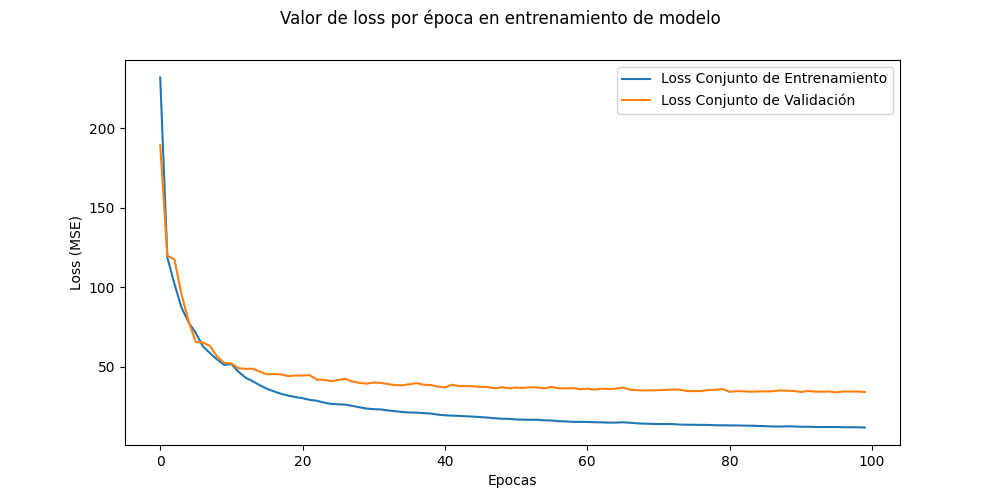
\includegraphics[width=1\linewidth]{images/results/exp1/delightpt.png}
    \caption{Curvas de aprendizaje en el entrenamiento del modelo \textit{DelightPt}}
    \label{fig:training-curves-delightpt}
\end{figure}

\section{Exploración de arquitecturas preentrenadas} \label{results:pretrained}
\subsection{Desempeño de arquitecturas preentrenadas con respecto a DELIGHT}

La siguiente tabla presenta las métricas de desempeño de los distintos experimentos realizados sobre arquitecturas preentrenadas, donde \textit{Original} corresponde a los resultados del trabajo de \cite{delight}, \textit{DelightPt} corresponde al modelo replicado en PyTorch y los modelos \textit{DR50}, \textit{DR50FT+ImageNet} y \textit{DR50FE+ImageNet} hacen alusión a los modelos Delight Resnet 50, Delight Resnet50 con Fine Tuning basado en ImageNet y Delight Resnet50 con Feature Extration basado en ImageNet, descritos en la sección \ref{methods:pretrained_arc}.\par\null\par

De manera similar a los resultados de la sección \ref{results:replication}, las métricas medidas son las descritas en la sección \ref{methods:metrics} correspondientes a las métricas de \textit{Root Mean Square Error (RMSE)} de la ecuación \ref{eq:rmse}, \textit{Desviación Media} de la ecuación \ref{eq:mean_deviation}, \textit{Desviación Mediana} de la ecuación \ref{eq:median_deviation} y \textit{Desviación Moda} de la ecuación \ref{eq:mode_deviation}.\par\null\par

\begin{table}[h]
    \centering
    \resizebox{17cm}{!} {
        \begin{tabular}{|c|c|c|c|c|c|}
            \hline
            Metricas & Original & DelightPt & DR50 & DR50FT+ImageNet & DR50FE+ImageNet \\ \hline
            RMSE & $\textbf{1.836} \pm 0.186^{\prime \prime}$ & $1.912 \pm 0.212^{\prime \prime}$ & $3.489 \pm 0.245^{\prime \prime}$ & $3.224 \pm 0.265^{\prime \prime}$ & $7.023 \pm 0.197^{\prime \prime}$\\ \hline
            Mean Deviation & $\textbf{0.783} \pm 0.009^{\prime \prime}$ & $0.805 \pm 0.025^{\prime \prime}$ & $1.408 \pm 0.047^{\prime \prime}$ & $1.232 \pm 0.044^{\prime \prime}$ & $4.391 \pm 0.079^{\prime \prime}$ \\ \hline
            Median Deviation & $0.468 \pm 0.008^{\prime \prime}$ & $\textbf{0.466} \pm 0.005^{\prime \prime}$ & $0.763 \pm 0.012^{\prime \prime}$ & $0.664 \pm 0.008^{\prime \prime}$ & $2.698 \pm 0.058^{\prime \prime}$ \\ \hline
            Mode Deviation & $0.427 \pm 0.051^{\prime \prime}$ & $0.427 \pm 0.043^{\prime \prime}$ & $\textbf{0.377} \pm 0.076^{\prime \prime}$ & $0.528 \pm 0.090^{\prime \prime}$ & $1.080 \pm 0.174^{\prime \prime}$ \\ \hline
        \end{tabular}
    }
    \caption{Comparación entre los modelos preentrenados, donde \textbf{Baseline} corresponde a un modelo ResNet50 entrenado desde cero, \textbf{FT+ImageNet} corresponde a un Fine Tuning del modelo ResNet50 preentrenado en ImageNet, y \textbf{FE+ImageNet} corresponde a un Feature Extraction del modelo ResNet50 preentrenado en ImageNet}
    \label{tab:pretrained_comparison}
\end{table}


\begin{figure}[h]
    \centering
    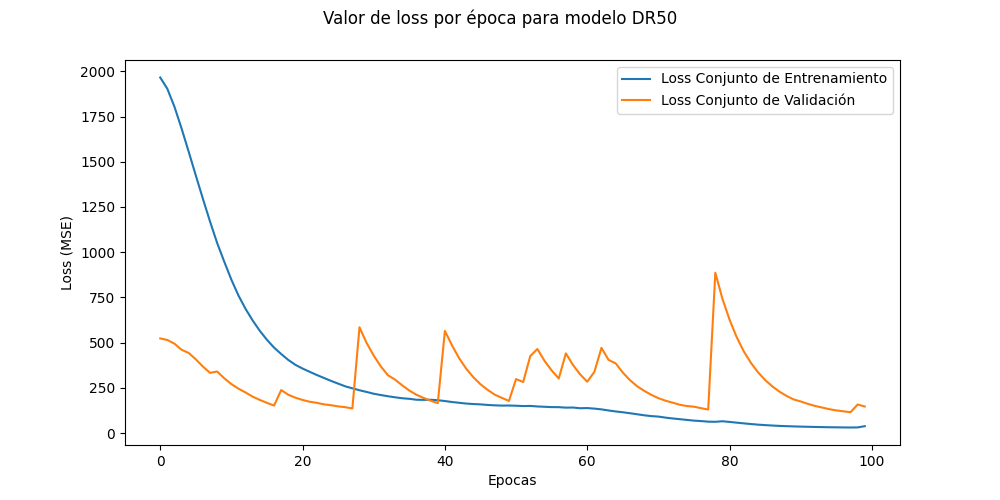
\includegraphics[width=1\linewidth]{images/results/exp1/dr50.png}
    \caption{Curvas de aprendizaje en el entrenamiento del modelo \textit{DR50}}
    \label{fig:training-curves-dr50}
\end{figure}

\begin{figure}[h]
    \centering
    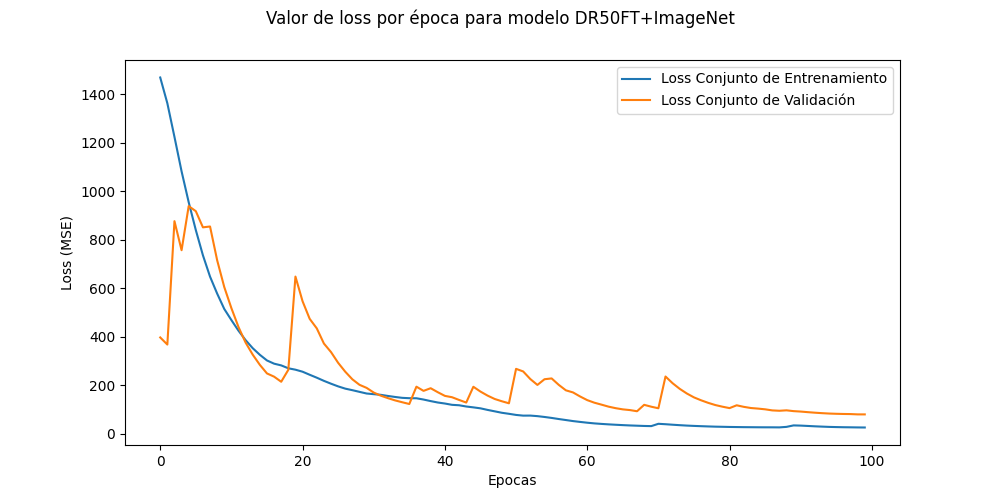
\includegraphics[width=1\linewidth]{images/results/exp1/dr50ft+ImageNet.png}
    \caption{Curvas de aprendizaje en el entrenamiento del modelo \textit{DR50FT+ImageNet}}
    \label{fig:training-curves-dr50ft+ImageNet}
\end{figure}

\begin{figure}[h!]
    \centering
    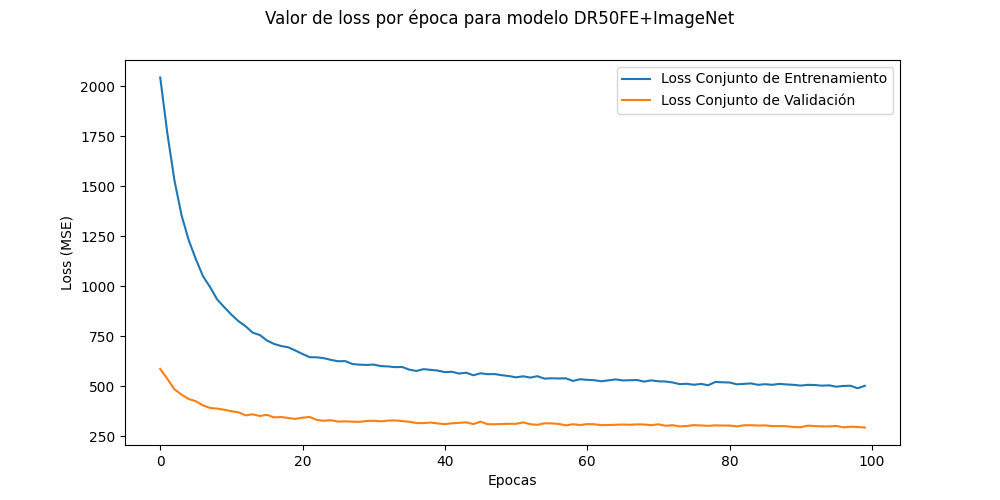
\includegraphics[width=1\linewidth]{images/results/exp1/dr50fe+ImageNet.png}
    \caption{Curvas de aprendizaje en el entrenamiento del modelo \textit{DR50FE+ImageNet}}
    \label{fig:training-curves-dr50fe+ImageNet}
\end{figure}

\section{Multimodalidad} \label{results:multimodality}
En esta sección se presentan las métricas de desempeño para el modelo multimodal titulado como \textit{DelightPt+Multiband}, usando como base el modelo propuesto en \cite{delight} y el modelo replicado en PyTorch \textit{DelightPt}. De igual forma que en los experimentos anteriores, las métricas medidas son las descritas en la sección \ref{methods:metrics} correspondientes a las métricas de \textit{Root Mean Square Error (RMSE)} de la ecuación \ref{eq:rmse}, \textit{Desviación Media} de la ecuación \ref{eq:mean_deviation}, \textit{Desviación Mediana} de la ecuación \ref{eq:median_deviation} y \textit{Desviación Moda} de la ecuación \ref{eq:mode_deviation}.\par\null\par

A su vez, se presenta un gráfico de comparación de dispersión de la métrica $MSE$ en el conjunto de evaluación, para el modelo original, \textit{DelightPt} y \textit{DelightPt+Multiband} \par\null\par

\begin{table}[ht]
    \centering
    \begin{tabular}{|c|c|c|c|}
        \hline
        Metricas & Original & DelightPt & DelightPt+Multiband \\ \hline
        RMSE & $\textbf{1.836} \pm 0.186^{\prime \prime}$ & $1.912 \pm 0.212^{\prime \prime}$ & $1.967 \pm 0.201^{\prime \prime}$ \\ \hline
        Mean Deviation & $0.783 \pm 0.009^{\prime \prime}$ & $0.805 \pm 0.025^{\prime \prime}$ & $\textbf{0.628} \pm 0.027^{\prime \prime}$ \\ \hline
        Median Deviation & $0.468 \pm 0.008^{\prime \prime}$ & $0.466 \pm 0.005^{\prime \prime}$ & $\textbf{0.269} \pm 0.004^{\prime \prime}$ \\ \hline
        Mode Deviation & $0.427 \pm 0.051^{\prime \prime}$ & $0.427 \pm 0.043^{\prime \prime}$ & $\textbf{0.126} \pm 0.015^{\prime \prime}$ \\ \hline
    \end{tabular}
    \caption{Comparación entre los resultados obtenidos en el trabajo original de \cite{delight} (bajo el nombre \textbf{Original}), \textbf{DelightPt} y el modelo multibanda \textbf{DelightPt+Multiband}}
    \label{tab:multiband_comparison}
\end{table}

\begin{figure}[h]
    \centering
    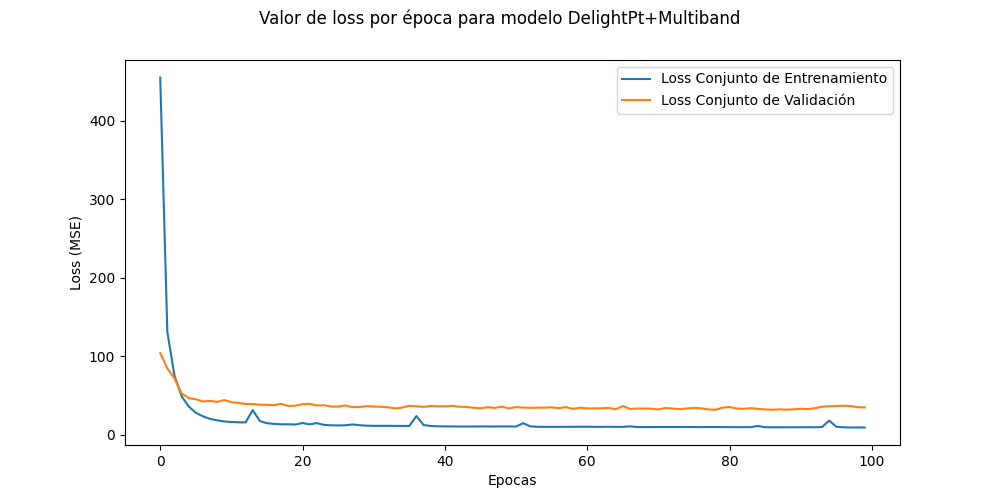
\includegraphics[width=1\linewidth]{delightpt+multiband.png}
    \caption{Curvas de aprendizaje en el entrenamiento del modelo \textit{DelightPt+Multiband}}
    \label{fig:training-curves-delightpt+multiband}
\end{figure}

\begin{figure}[!ht]
    \centering
    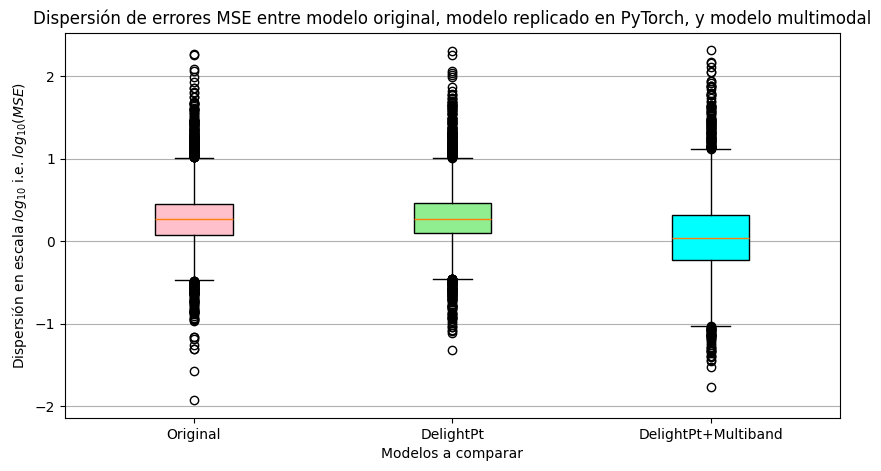
\includegraphics[width=0.8\linewidth]{images//results/delightpt+multiband_dispersion.png}
    \caption{Gráfico de dispersión de los resultados de la tabla \ref{tab:multiband_comparison}}
    \label{fig:graph-multiband}
\end{figure}

\section{Domain Adaptation} \label{results:transfer-learning}
En ésta ultima sección, se presentan las métricas de desempeño del modelo \textit{DelightPt} del experimento \ref{methods:replication}, evaluado en las distintas bandas de la fuente de datos \ref{methods:dataset2}, para así evaluar la capacidad de adaptación a un nuevo dominio de cara a los nuevos datos que se disponibilizarán gracias a la salida de los telescopios en construcción.\par\null\par

Como se mencionó en los resultados anteriores, las métricas medidas son las descritas en la sección \ref{methods:metrics} correspondientes a las métricas de \textit{Root Mean Square Error (RMSE)} de la ecuación \ref{eq:rmse}, \textit{Desviación Media} de la ecuación \ref{eq:mean_deviation}, \textit{Desviación Mediana} de la ecuación \ref{eq:median_deviation} y \textit{Desviación Moda} de la ecuación \ref{eq:mode_deviation}.\par\null\par

A su vez, se presenta un gráfico de comparación de dispersión de la métrica $MSE$ en el conjunto de evaluación, para las distintas bandas analizadas\par\null\par

% agrupar por columnas
\subsection{Comparación entre bandas}
\begin{table}[ht]
    \centering
    \resizebox{17cm}{!} {
        \begin{tabular}{|c|c|c|c|c|c|c|c|}
        \hline
        Métricas         & Original & DelightPt                               & g-band                          & r-band                          & i-band                                   & z-band                                   & y-band                          \\ \hline
        RMSE             & $\textbf{1.836} \pm 0.186^{\prime \prime}$ & $1.912 \pm 0.212^{\prime \prime}$ & $7.400 \pm 0.276^{\prime \prime}$ & $2.612 \pm 0.276^{\prime \prime}$ & $2.433 \pm 0.228^{\prime \prime}$          & $2.575 \pm 0.274^{\prime \prime}$          & $3.059 \pm 0.265^{\prime \prime}$ \\ \hline
        Mean Deviation   & $0.783 \pm 0.009^{\prime \prime}$ & $0.805 \pm 0.025^{\prime \prime}$          & $2.835 \pm 0.098^{\prime \prime}$ & $0.747 \pm 0.037^{\prime \prime}$ & $0.784 \pm 0.034^{\prime \prime}$          & $\textbf{0.712} \pm 0.036^{\prime \prime}$ & $0.907 \pm 0.043^{\prime \prime}$ \\ \hline
        Median Deviation & $0.468 \pm 0.008^{\prime \prime}$ & $0.466 \pm 0.005^{\prime \prime}$          & $0.461 \pm 0.012^{\prime \prime}$ & $0.287 \pm 0.005^{\prime \prime}$ & $0.288 \pm 0.005^{\prime \prime}$          & $\textbf{0.282} \pm 0.005^{\prime \prime}$ & $0.311 \pm 0.006^{\prime \prime}$ \\ \hline
        Mode Deviation   & $0.427 \pm 0.051^{\prime \prime}$ & $0.427 \pm 0.043^{\prime \prime}$          & $0.176 \pm 0.025^{\prime \prime}$ & $0.176 \pm 0.028^{\prime \prime}$ & $\textbf{0.126} \pm 0.014^{\prime \prime}$ & $0.126 \pm 0.022^{\prime \prime}$          & $0.176 \pm 0.024^{\prime \prime}$ \\ \hline
    \end{tabular}
    }
    \caption{Comparaciones entre distintas evaluaciones de DelightPt, donde \textit{Original} corresponde a los resultados obtenidos en el trabajo de \cite{delight}, \textit{Control} representa la evaluación en el dataset \ref{methods:dataset1}, y el resto de columnas \textit{$k$-band} es el resultado de evaluar el modelo de \textit{DelightPt}, entrenado en el dataset \ref{methods:dataset1}, en el dataset \ref{methods:dataset2} respecto a la banda $k$, con $k \in \{g, r, 
 i, z, y\}$}
    \label{tab:transfer_learning}
\end{table}

\begin{figure}[ht]
    \centering
    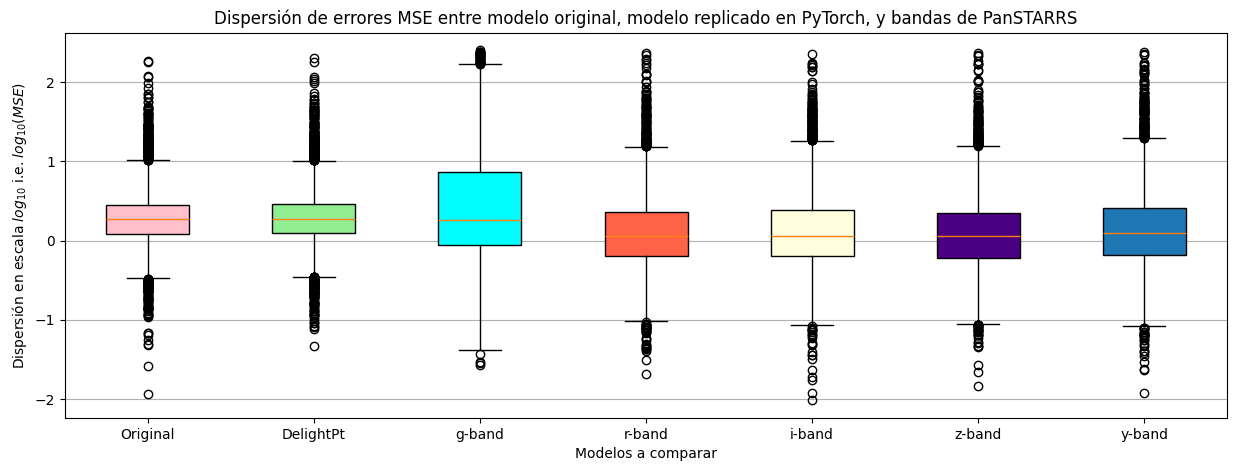
\includegraphics[width=1\linewidth]{images/results/delight_dispersion_bands.png}
    \caption{Gráfico de dispersión de los resultados de la tabla \ref{tab:transfer_learning}}
    \label{fig:graph-transfer-learning}
\end{figure}


\end{document}  